
\section{AIG CDS data over 2005 \& 2010}
\label{sec:aig-cds-data}

In this section we will apply the previous results on datas provided by AIG.

In the paper \cite{OTRATS}, A.cousin \& I.Niang showed that the CDS market contains
no  arbitration   opportunity  if   credit  curve   is  a   default  distribution
function witch implied that this function must be a decreasing function.\\
Among  the period  16/08/2005 -  28/09/2007  we can  see that  the credit  curve
appears to be non decreasing :

\begin{figure}[H]
  \centering
  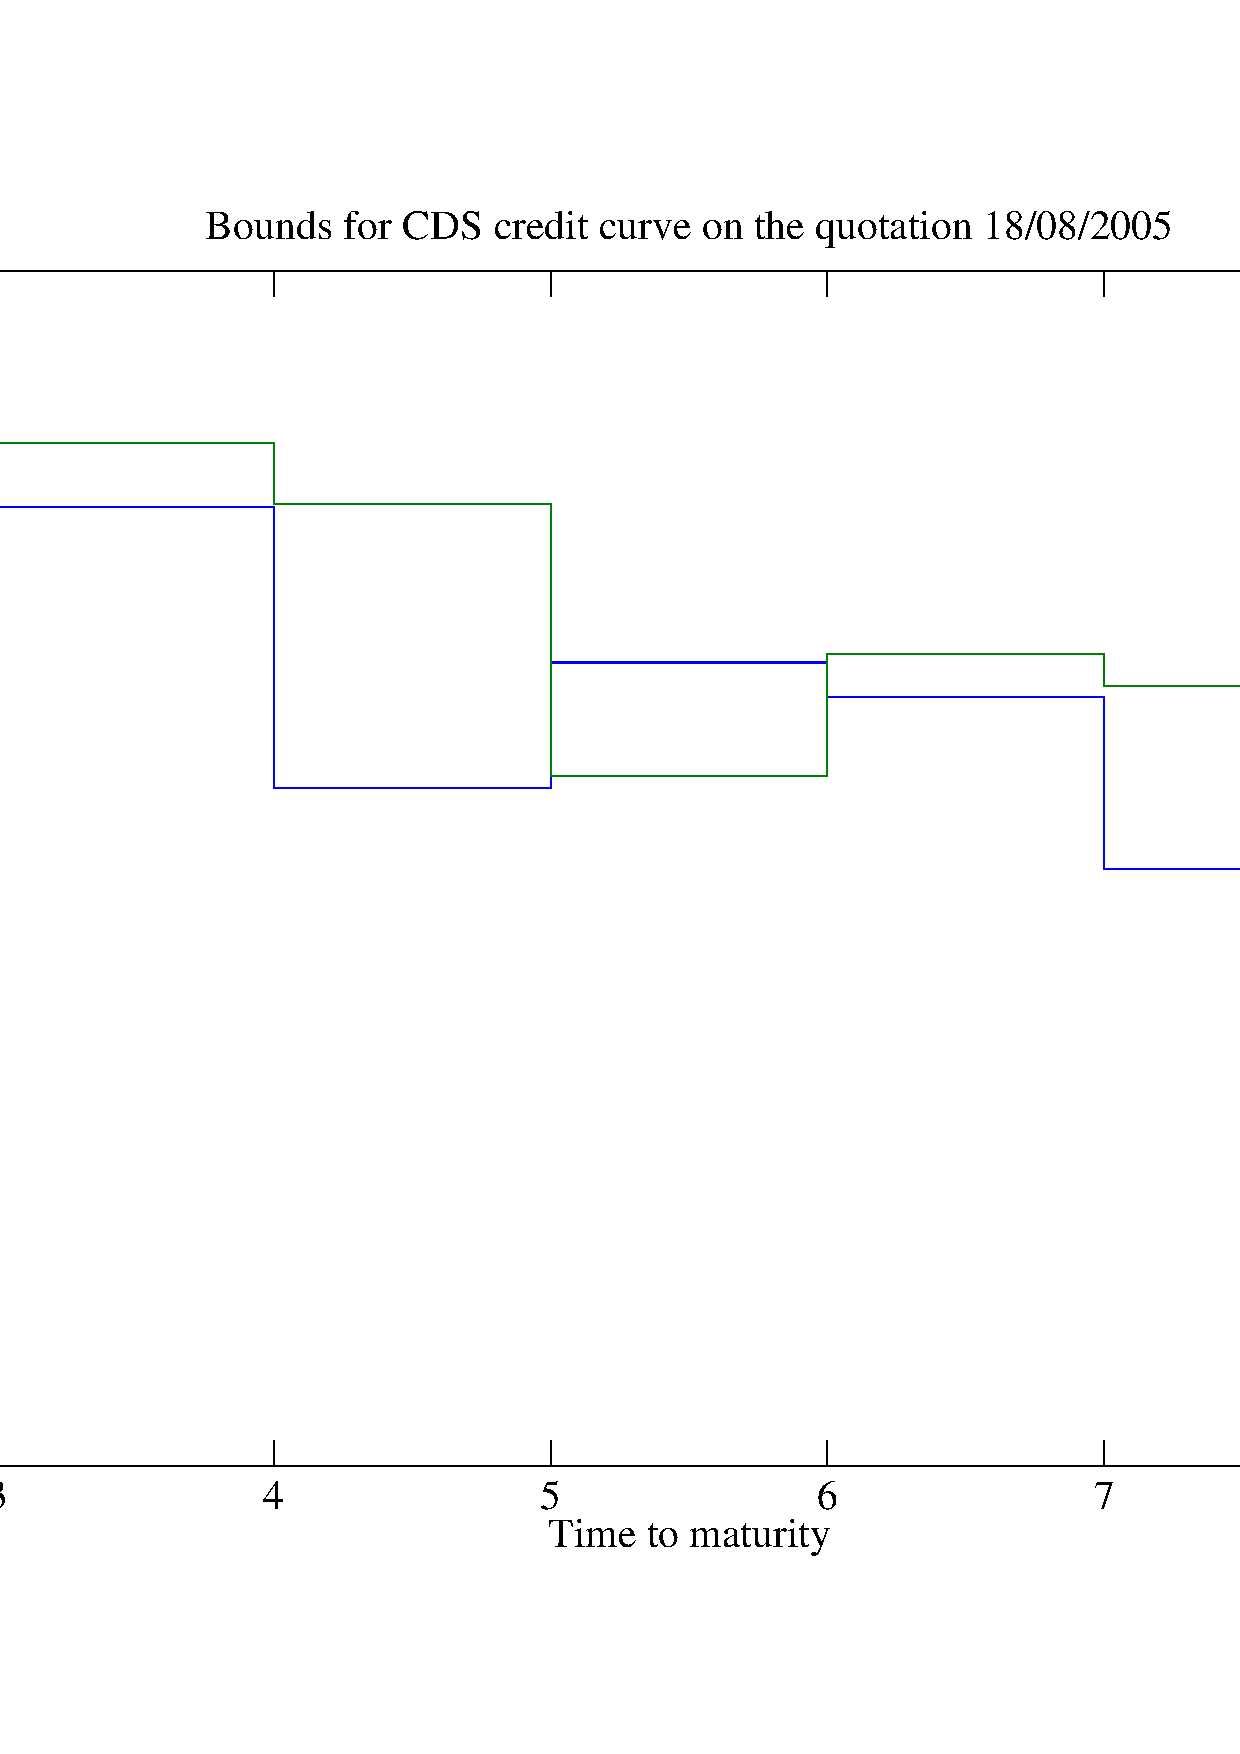
\includegraphics[width=0.8\textwidth]{cotation-18-08-2005.pdf}
  \caption{Credit curve among 18/08/2005 -  28/09/2007}
\end{figure}
\\
Since 28/09/2007 we can see that the  credit curve fit well the market condition
:


\begin{figure}[H]
  \centering
  \includegraphics[width=0.8\textwidth]{cotation27-11-2007.pdf}
  \caption{Credit curve since 28/09/2007 : here in 27/11/2007}
\end{figure}


